% 2008 年北京卷文科第 13 题：函数 f(x) 的图象为折线段 ABC。
% 来源 PDF：普通高考/2008/2008北京文.pdf，SHA256 9d725e3f7011f50eddddd9bebd62825365c218b08fa0c920ac23b57228f590f9
% 原页：第 1 页（A3 三栏）第 2 栏中部，印刷页 427。
% 重绘依据：坐标轴 x=0..6、y=0..4；单位网格线；折线 A(0,4)—B(2,0)—C(6,4)；
%   A、B、C 三点标注与原图一致。
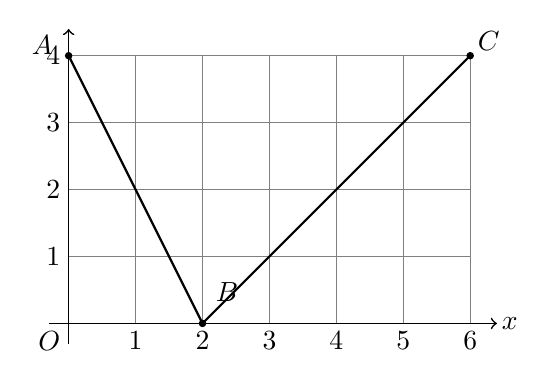
\begin{tikzpicture}[scale=0.85, semithick, every node/.style={inner sep=1.5pt}]
  % 网格
  \draw[help lines, step=1] (0,0) grid (6,4);
  % 坐标轴
  \draw[->] (-0.3,0) -- (6.4,0) node[anchor=west] {$x$};
  \draw[->] (0,-0.3) -- (0,4.4);
  \node[anchor=north east] at (-0.05,-0.05) {$O$};
  \foreach \x in {1,2,3,4,5,6} \node[anchor=north] at (\x,-0.05) {$\x$};
  \foreach \y in {1,2,3,4} \node[anchor=east] at (-0.05,\y) {$\y$};
  % 折线
  \draw[thick] (0,4) -- (2,0) -- (6,4);
  \fill (0,4) circle (1.6pt) node[anchor=east, xshift=-4pt, yshift=4pt] {$A$};
  \fill (2,0) circle (1.6pt) node[anchor=south west, xshift=3pt, yshift=6pt] {$B$};
  \fill (6,4) circle (1.6pt) node[anchor=south west, xshift=1pt] {$C$};
\end{tikzpicture}
